\documentclass[12pt, a4paper]{article}
\usepackage{ctex} % 支持中文处理
\usepackage{geometry} % 页面布局
\usepackage{graphicx} % 图片支持
\usepackage{hyperref} % 超链接支持
\usepackage{amsmath} % 数学公式
\usepackage{amsfonts}
\usepackage{amssymb}
\usepackage{amsthm}
\usepackage{bm}
\usepackage{color}
\usepackage{physics}
\usepackage{subcaption}
\usepackage{media9}
\usepackage{hyperref}

\geometry{left=2.5cm,right=2.5cm,top=2.5cm,bottom=2.5cm} % 设置页边距
\title{结果讨论}
\author{安庭毅\ 工学院 \ 2100011014}
\date{\today} % 使用今天的日期

\begin{document}

\maketitle % 显示标题
\section{稳定性分析}
对于一阶迎风格式,蛙跳格式和LaxWendroff,固定空间格点数为301, 分别考察CFL数为0.9,1.0,1.1时推进到T=1.0,1.25和2.0时的数值计算结果。

\begin{figure}[htbp]
    \centering
    \begin{subfigure}[b]{0.45\textwidth} 
        \centering
        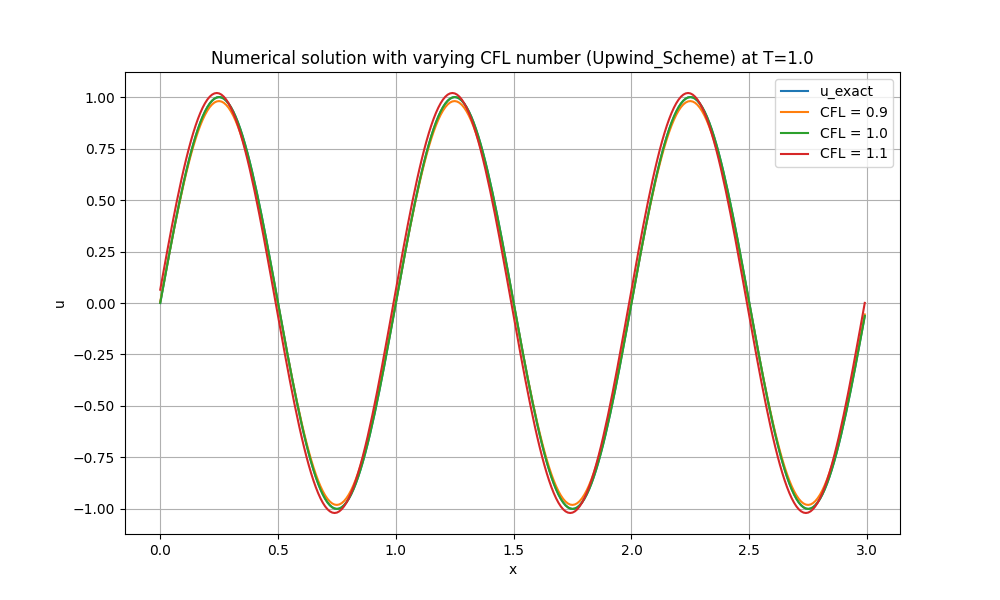
\includegraphics[width=\textwidth]{./pictures/Stablity_of_Upwind_Scheme_at_1.0.png} 
    \end{subfigure}
    \hfill
    \begin{subfigure}[b]{0.45\textwidth} 
        \centering
        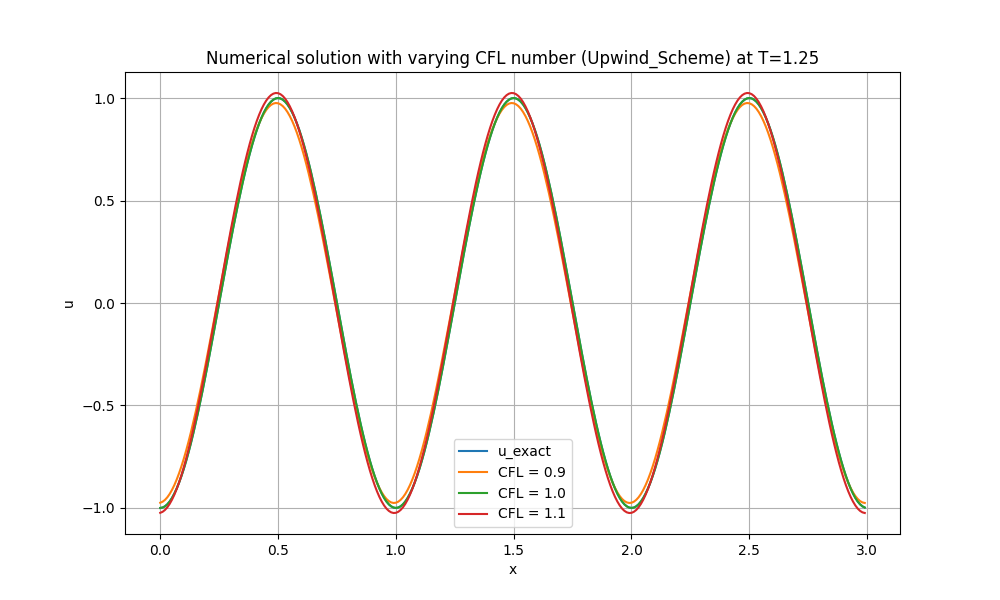
\includegraphics[width=\textwidth]{./pictures/Stablity_of_Upwind_Scheme_at_1.25.png} 
    \end{subfigure}
    \vspace{0.5cm}
    \centering
    \begin{subfigure}[b]{0.45\textwidth} 
        \centering
        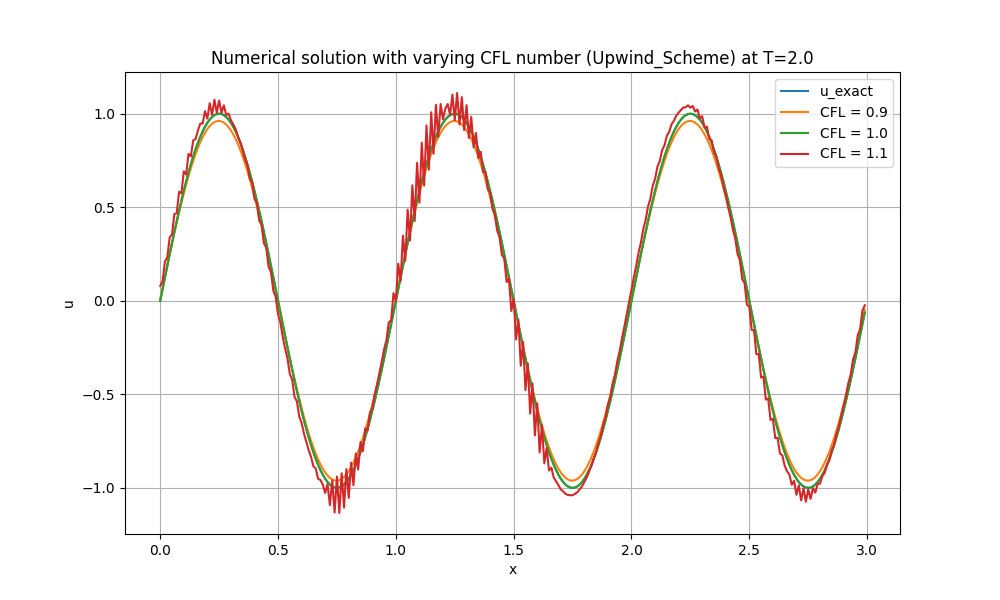
\includegraphics[width=\textwidth]{./pictures/Stablity_of_Upwind_Scheme_at_2.0.png} 
    \end{subfigure}
    \caption{一阶迎风格式的计算结果}
\end{figure}

\begin{figure}[htbp]
    \centering
    \begin{subfigure}[b]{0.45\textwidth} 
        \centering
        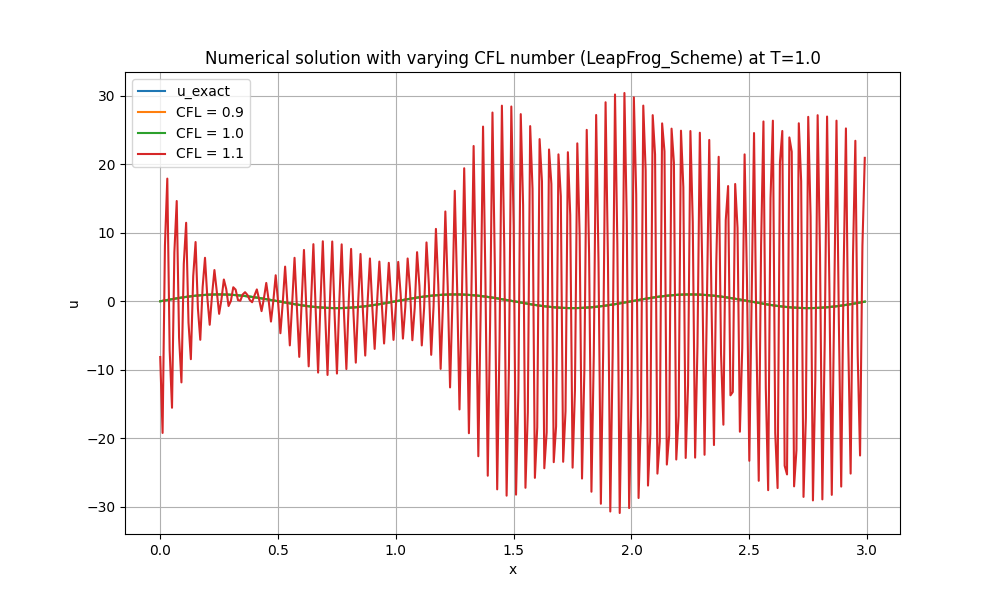
\includegraphics[width=\textwidth]{./pictures/Stablity_of_LeapFrog_Scheme_at_1.0.png} 
    \end{subfigure}
    \hfill
    \begin{subfigure}[b]{0.45\textwidth} 
        \centering
        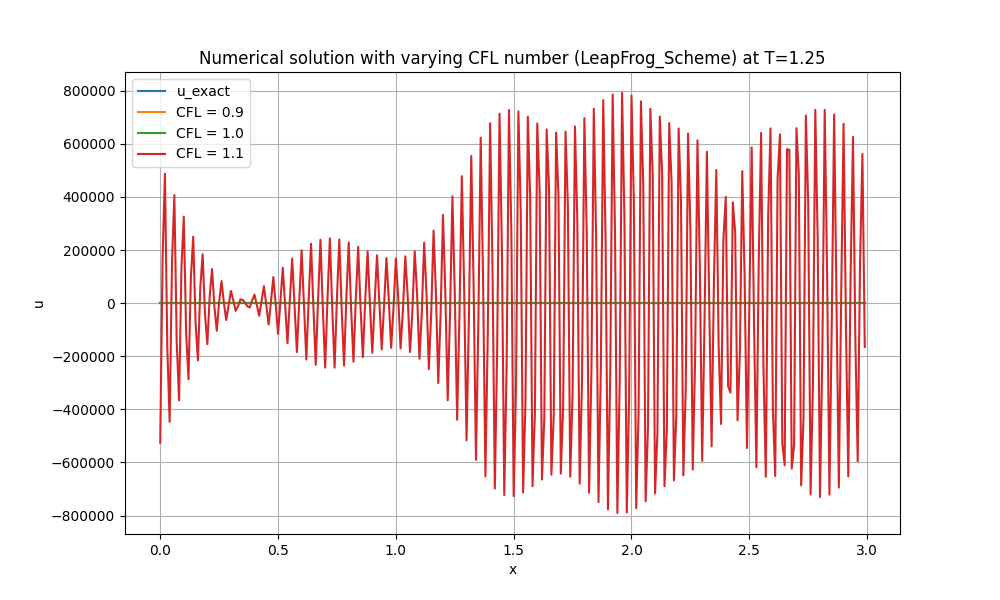
\includegraphics[width=\textwidth]{./pictures/Stablity_of_LeapFrog_Scheme_at_1.25.png} 
    \end{subfigure}
    \vspace{0.5cm}
    \centering
    \begin{subfigure}[b]{0.45\textwidth} 
        \centering
        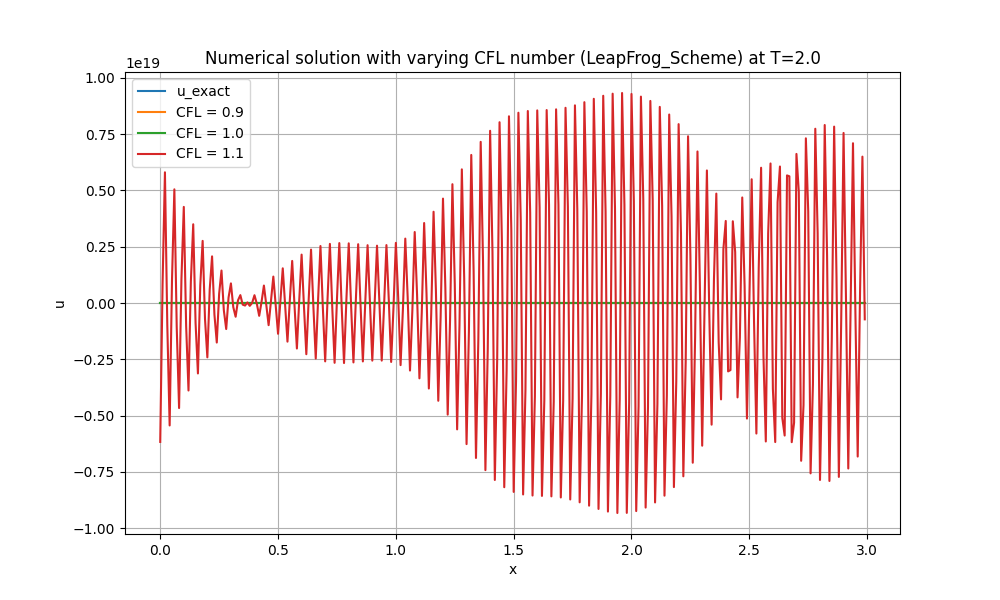
\includegraphics[width=\textwidth]{./pictures/Stablity_of_LeapFrog_Scheme_at_2.0.png} 
    \end{subfigure}
    \caption{蛙跳格式的计算结果}
\end{figure}

\begin{figure}[htbp]
    \centering
    \begin{subfigure}[b]{0.45\textwidth} 
        \centering
        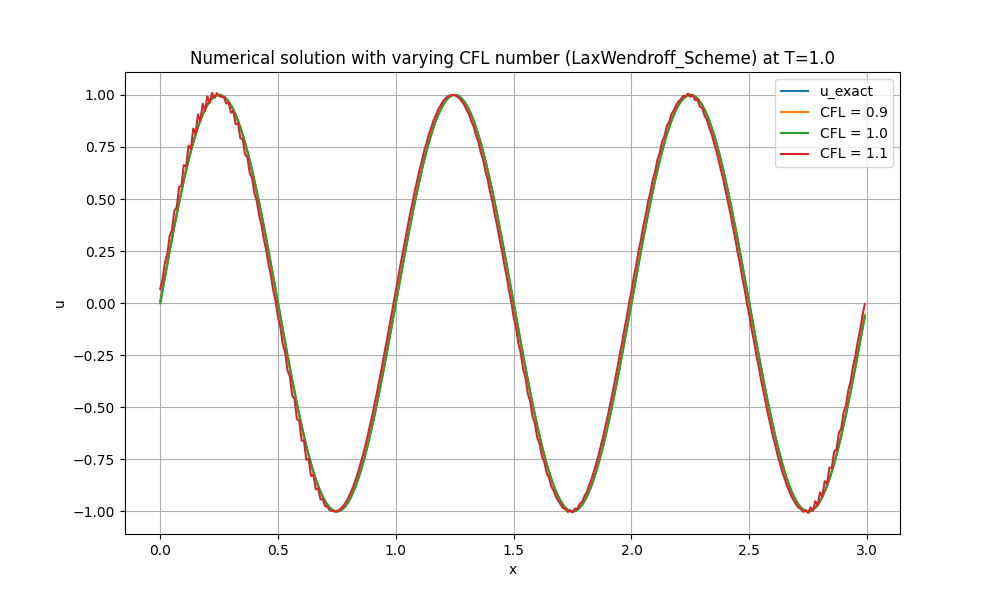
\includegraphics[width=\textwidth]{./pictures/Stablity_of_LaxWendroff_Scheme_at_1.0.png} 
    \end{subfigure}
    \hfill
    \begin{subfigure}[b]{0.45\textwidth} 
        \centering
        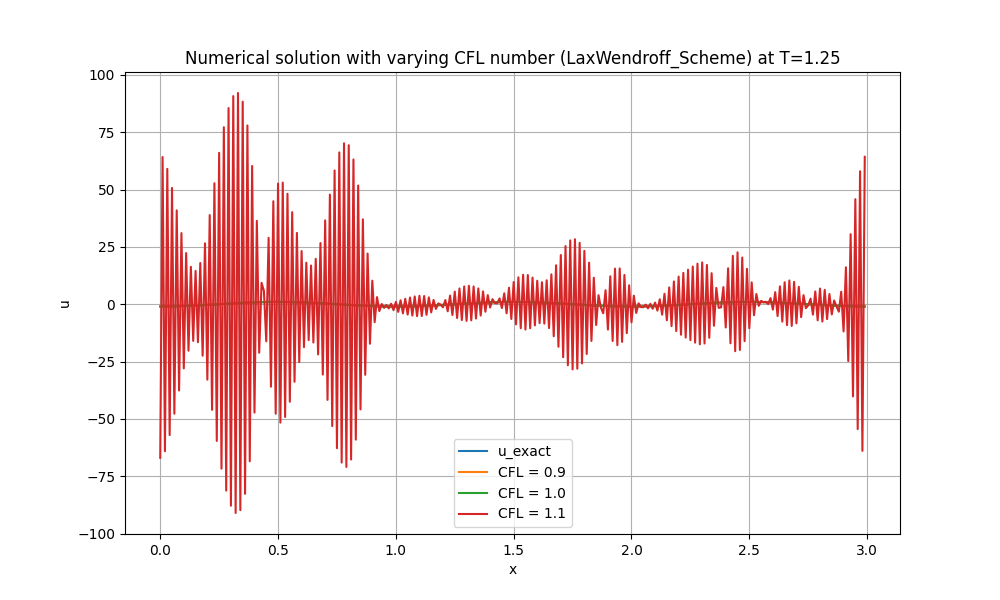
\includegraphics[width=\textwidth]{./pictures/Stablity_of_LaxWendroff_Scheme_at_1.25.png} 
    \end{subfigure}
    \vspace{0.5cm}
    \centering
    \begin{subfigure}[b]{0.45\textwidth} 
        \centering
        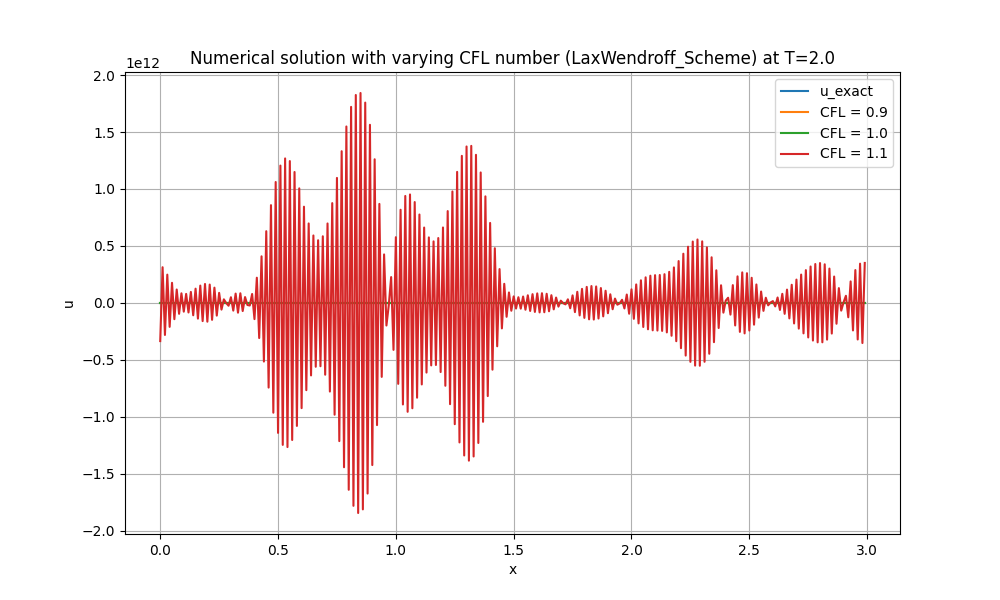
\includegraphics[width=\textwidth]{./pictures/Stablity_of_LaxWendroff_Scheme_at_2.0.png} 
    \end{subfigure}
    \caption{LaxWendroff格式的计算结果}
\end{figure}

对于一阶迎风格式,可以看出CFL=1.1时,时间推进到2.0时数值解出现明显波动。这与理论分析结果相符。注意到此时的数值解已有耗散现象。

对于蛙跳格式和LaxWendroff格式,在CFL=1.1时,时间推进到1.25已出现明显发散。这与理论分析一致,一定程度说明了相比于一阶迎风格式二者对CFL数的敏感性。

\subsection{精度分析}
对于三种格式,均采用离散$L_2$范数衡量误差。默认CFL数为0.8,时间推进到T=1.0,逐渐分半加密空间网格计算收敛阶。
\begin{figure}[htbp]
    \centering
    \begin{subfigure}[b]{0.45\textwidth} 
        \centering
        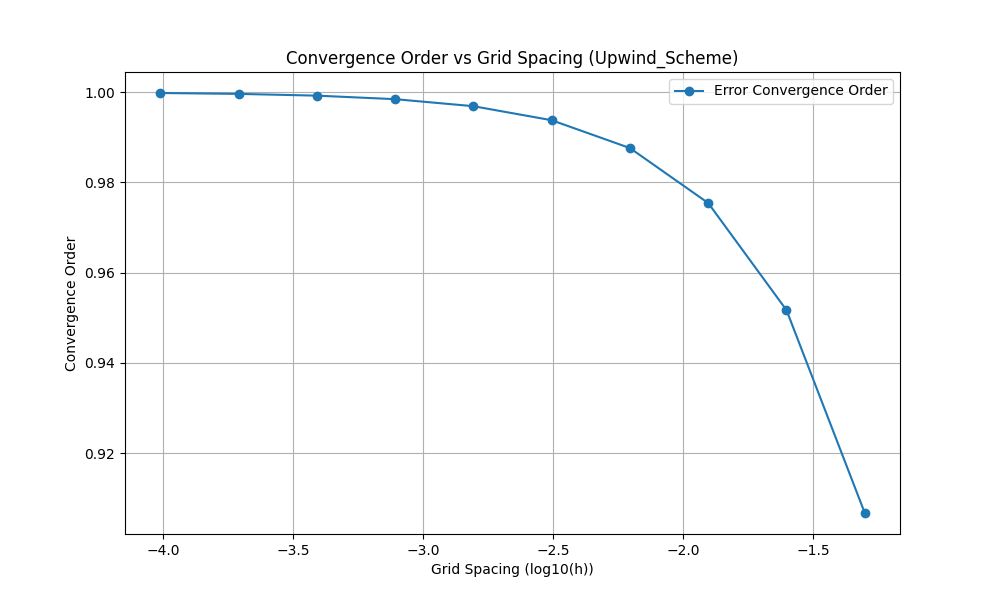
\includegraphics[width=\textwidth]{./pictures/Convergence_Order_of_Upwind_Scheme.png} 
    \end{subfigure}
    \hfill
    \begin{subfigure}[b]{0.45\textwidth} 
        \centering
        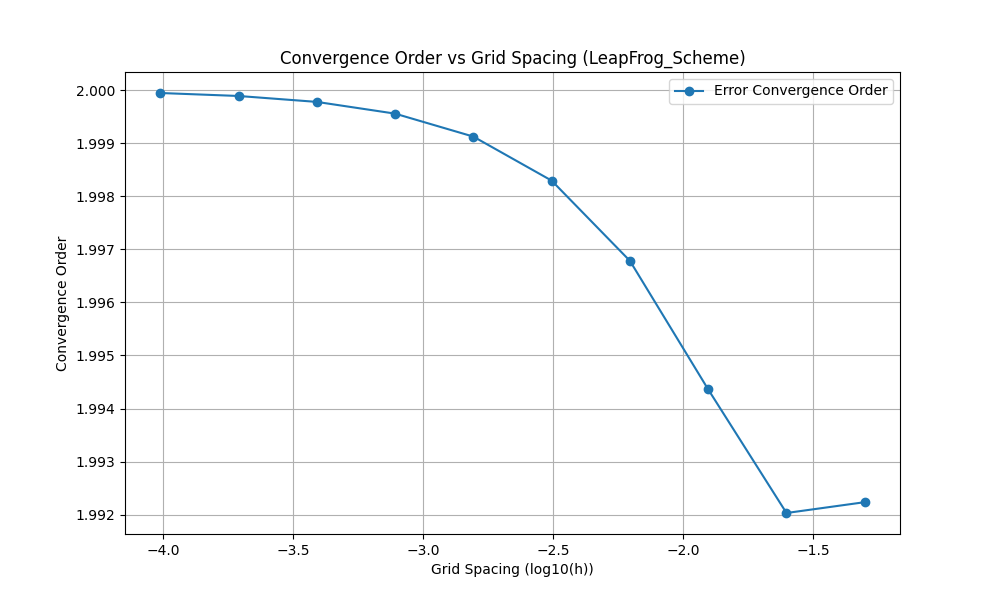
\includegraphics[width=\textwidth]{./pictures/Convergence_Order_of_LeapFrog_Scheme.png} 
    \end{subfigure}
    \vspace{0.5cm}
    \centering
    \begin{subfigure}[b]{0.45\textwidth} 
        \centering
        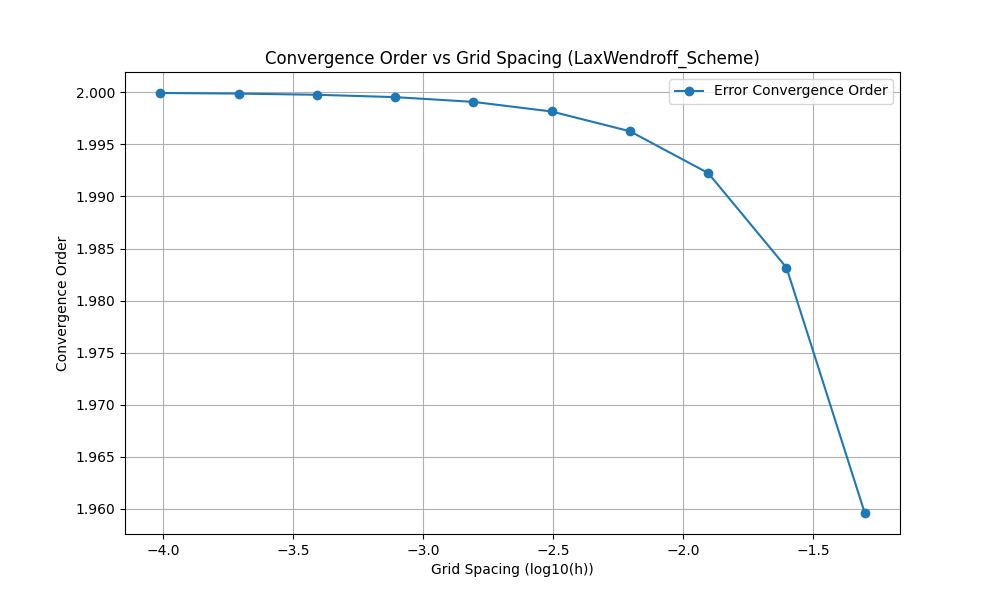
\includegraphics[width=\textwidth]{./pictures/Convergence_Order_of_LaxWendroff_Scheme.png} 
    \end{subfigure}
    \caption{三种格式收敛阶分析}
\end{figure}
与理论分析均一致。

\section{耗散与色散分析}
在时间步长固定为0.01时,时间推进到T=100.0,CFL数设置为0.8,观察数值解的演化情况:\\
\href{run:./pictures/solution_evolution_of_Upwind_Scheme.mp4}{播放:一阶迎风格式数值解的演化}\\
\href{run:./pictures/solution_evolution_of_LeapFrog_Scheme.mp4}{播放:蛙跳格式数值解的演化}\\
\href{run:./pictures/solution_evolution_of_LaxWendroff_Scheme.mp4}{播放:LaxWendroff格式数值解的演化}\\

可以看到,随时间推进,一阶迎风格式的数值解出现明显的耗散,解的振幅减小;而蛙跳格式和LaxWendroff格式均出现明显的相位滞后。这与理论分析一致(迎风格式耗散主导,蛙跳格式和LaxWendroff格式色散主导)。

\section*{附1:AI工具使用说明表}
使用的AI工具:deepseek和GPT-4o

AI生成代码行数及功能:numerical\_test.py中31-38,56-64,76-86行由AI生成,均为画图功能

核心代码自主编写比例:81\%

\section*{附2:git版本控制记录}
\begin{figure}[htbp]
    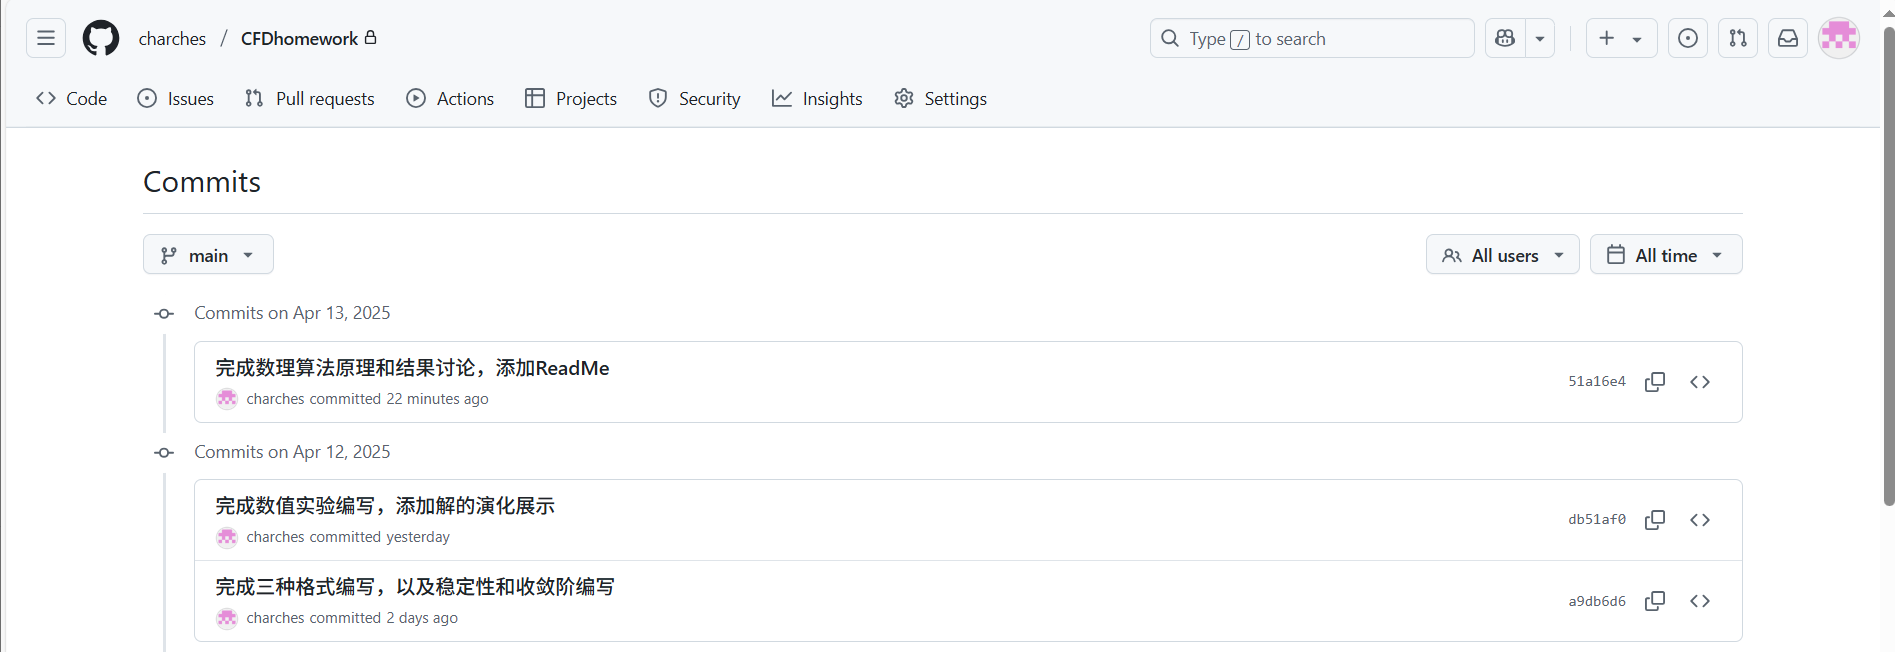
\includegraphics[width=0.8\textwidth]{./pictures/git_control.png}
\end{figure}
\end{document}